
% This LaTeX was auto-generated from MATLAB code.
% To make changes, update the MATLAB code and republish this document.

\documentclass{article}
\usepackage{graphicx}
\usepackage{color}

\sloppy
\definecolor{lightgray}{gray}{0.5}
\setlength{\parindent}{0pt}

\begin{document}

    
    
\subsection*{Contents}

\begin{itemize}
\setlength{\itemsep}{-1ex}
   \item Initialization and model definition
   \item Generate system matrixes for linear model
   \item Solve QP problem with linear model
   \item Extract control inputs and states
   \item Plotting
   \item LQR
\end{itemize}
\begin{verbatim}
% TTK4135 - Helicopter lab
% Hints/template for problem 2.
% Updated spring 2017, Andreas L. Fl?ten
\end{verbatim}


\subsection*{Initialization and model definition}

\begin{verbatim}
code42; % NB: Change this to the init file corresponding to your helicopter

global N mx

% Discrete time system model. x = [lambda r p p_dot e e_dot]'
A1 = A;
B1 = B;

% Number of states and inputs
mx = size(A1,2); % Number of states (number of columns in A)
mu = size(B1,2); % Number of inputs(number of columns in B)

% Initial values
x1_0 = pi;                               % Lambda
x2_0 = 0;                               % r
x3_0 = 0;                               % p
x4_0 = 0;                               % p_dot
x5_0 = 0;
x6_0 = 0;
x0 = [x1_0 x2_0 x3_0 x4_0 x5_0 x6_0]';          % Initial values

% Time horizon and initialization
N  = 80;                                % Time horizon for states
M  = N;                                 % Time horizon for inputs
z  = zeros(N*mx+M*mu,1);                % Initialize z for the whole horizon
z0 = z;                                 % Initial value for optimization

% Bounds
ul 	    = -30*pi/180;                   % Lower bound on control -- u1
uu 	    = 30*pi/180;                    % Upper bound on control -- u1

xl      = -Inf*ones(mx,1);              % Lower bound on states (no bound)
xu      = Inf*ones(mx,1);               % Upper bound on states (no bound)
xl(3)   = ul;                           % Lower bound on state x3
xu(3)   = uu;                           % Upper bound on state x3
%%xl(4)   = -0.1;                         % Lower bound on state x4
%%xu(4)   = 0.1;                          % Upper bound on state x4

% Generate constraints on measurements and inputs
[vlb,vub]       = hints_genbegr2(N,M,xl,xu,ul,uu);      % hint: genbegr2
vlb(N*mx+M*mu)  = 0;                                    % We want the last input to be zero
vub(N*mx+M*mu)  = 0;                                    % We want the last input to be zero

% Generate the matrix Q and the vector c (objecitve function weights in the QP problem)
Q1 = zeros(mx,mx);
Q1(1,1) = 1;                            % Weight on state x1
Q1(2,2) = 0;                            % Weight on state x2
Q1(3,3) = 0;                            % Weight on state x3
Q1(4,4) = 0;                            % Weight on state x4
Q1(5,5) = 0;                            % Weight on state x5
Q1(6,6) = 0;                            % Weight on state x6
q1 = 1;
q2 = 1;
P1 = hints_blkdiag(q1,q2);              % Weight on input
Q = 2*hints_genq2(Q1,P1,N,M,mu);        % Generate Q
%%c = zeros(N*mx+M*mu,1);                 % Generate c
\end{verbatim}


\subsection*{Generate system matrixes for linear model}

\begin{verbatim}
Aeq = hints_gena2(A1,B1,N,mx,mu);           % Generate A, hint: gena2
beq = [A1*x0; zeros((N-1)*mx,1)];
%%beq = zeros(mx*N, 2);                       % Generate b
%%beq(1:mx) = A1*x0;                          % Initial value

%User input
%G = hints_blkdiag(Q,c);
\end{verbatim}


\subsection*{Solve QP problem with linear model}

\begin{verbatim}
options = optimset('fmincon');
options.MaxFunEvals = 20000
options.Display = 'iter'
f = @(z) z'*Q*z;
tic
[z, fval] = fmincon(f,z0,[],[],Aeq,beq,vlb,vub,@func_constraint, options);
t1=toc;

% Calculate objective value
phi1 = 0.0;
PhiOut = zeros(N*mx+M*mu,1);
for i=1:N*mx+M*mu
  phi1=phi1+Q(i,i)*z(i)*z(i);
  PhiOut(i) = phi1;
end
\end{verbatim}

        \color{lightgray} \begin{verbatim}
options = 

                   Display: 'final'
               MaxFunEvals: 20000
                   MaxIter: []
                    TolFun: 1.0000e-06
                      TolX: []
               FunValCheck: 'off'
                 OutputFcn: []
                  PlotFcns: []
           ActiveConstrTol: []
                 Algorithm: 'interior-point'
    AlwaysHonorConstraints: 'bounds'
           DerivativeCheck: 'off'
               Diagnostics: 'off'
             DiffMaxChange: Inf
             DiffMinChange: 0
            FinDiffRelStep: []
               FinDiffType: 'forward'
         GoalsExactAchieve: []
                GradConstr: 'off'
                   GradObj: 'off'
                   HessFcn: []
                   Hessian: []
                  HessMult: []
               HessPattern: 'sparse(ones(numberofvariables))'
                HessUpdate: []
           InitialHessType: []
         InitialHessMatrix: []
          InitBarrierParam: 0.1000
     InitTrustRegionRadius: 'sqrt(numberofvariables)'
                  Jacobian: []
                 JacobMult: []
              JacobPattern: []
                LargeScale: []
                  MaxNodes: []
                MaxPCGIter: 'max(1,floor(numberofvariables/2))'
             MaxProjCGIter: '2*(numberofvariables-numberofequalities)'
                MaxSQPIter: '10*max(numberofvariables,numberofinequalities...'
                   MaxTime: []
             MeritFunction: []
                 MinAbsMax: []
        NoStopIfFlatInfeas: []
            ObjectiveLimit: -1.0000e+20
      PhaseOneTotalScaling: []
            Preconditioner: []
          PrecondBandWidth: 0
            RelLineSrchBnd: []
    RelLineSrchBndDuration: 1
              ScaleProblem: 'none'
                   Simplex: []
       SubproblemAlgorithm: 'ldl-factorization'
                    TolCon: 1.0000e-06
                 TolConSQP: 1.0000e-06
                TolGradCon: []
                    TolPCG: 0.1000
                 TolProjCG: 0.0100
              TolProjCGAbs: 1.0000e-10
                  TypicalX: 'ones(numberofvariables,1)'
               UseParallel: 0


options = 

                   Display: 'iter'
               MaxFunEvals: 20000
                   MaxIter: []
                    TolFun: 1.0000e-06
                      TolX: []
               FunValCheck: 'off'
                 OutputFcn: []
                  PlotFcns: []
           ActiveConstrTol: []
                 Algorithm: 'interior-point'
    AlwaysHonorConstraints: 'bounds'
           DerivativeCheck: 'off'
               Diagnostics: 'off'
             DiffMaxChange: Inf
             DiffMinChange: 0
            FinDiffRelStep: []
               FinDiffType: 'forward'
         GoalsExactAchieve: []
                GradConstr: 'off'
                   GradObj: 'off'
                   HessFcn: []
                   Hessian: []
                  HessMult: []
               HessPattern: 'sparse(ones(numberofvariables))'
                HessUpdate: []
           InitialHessType: []
         InitialHessMatrix: []
          InitBarrierParam: 0.1000
     InitTrustRegionRadius: 'sqrt(numberofvariables)'
                  Jacobian: []
                 JacobMult: []
              JacobPattern: []
                LargeScale: []
                  MaxNodes: []
                MaxPCGIter: 'max(1,floor(numberofvariables/2))'
             MaxProjCGIter: '2*(numberofvariables-numberofequalities)'
                MaxSQPIter: '10*max(numberofvariables,numberofinequalities...'
                   MaxTime: []
             MeritFunction: []
                 MinAbsMax: []
        NoStopIfFlatInfeas: []
            ObjectiveLimit: -1.0000e+20
      PhaseOneTotalScaling: []
            Preconditioner: []
          PrecondBandWidth: 0
            RelLineSrchBnd: []
    RelLineSrchBndDuration: 1
              ScaleProblem: 'none'
                   Simplex: []
       SubproblemAlgorithm: 'ldl-factorization'
                    TolCon: 1.0000e-06
                 TolConSQP: 1.0000e-06
                TolGradCon: []
                    TolPCG: 0.1000
                 TolProjCG: 0.0100
              TolProjCGAbs: 1.0000e-10
                  TypicalX: 'ones(numberofvariables,1)'
               UseParallel: 0

                                            First-order      Norm of
 Iter F-count            f(x)  Feasibility   optimality         step
    0     641    0.000000e+00    3.142e+00    4.130e-08
    1    1290    6.094652e-01    2.592e+00    2.229e-02    5.845e-01
    2    1935    5.259258e+00    1.552e+00    5.086e-02    1.173e+00
    3    2579    6.137941e+00    1.494e+00    3.567e-01    4.432e-01
    4    3220    1.458992e+01    1.277e+00    6.493e-01    1.797e+00
    5    3861    2.022316e+01    1.189e+00    9.959e-01    7.250e-01
    6    4503    2.023725e+01    1.189e+00    9.964e-01    1.683e-03
    7    5144    2.025145e+01    1.189e+00    9.968e-01    1.706e-03
    8    5785    2.597526e+01    1.083e+00    5.154e-01    1.069e+00
    9    6426    4.598311e+01    8.437e-01    5.919e+00    3.155e+00
   10    7067    4.436232e+01    7.832e-01    5.905e+00    2.490e+00
   11    7708    4.324773e+01    7.661e-01    5.899e+00    1.145e+00
   12    8349    4.307538e+01    7.487e-01    5.890e+00    9.732e-01
   13    8990    4.658664e+01    7.063e-01    5.887e+00    1.504e+00
   14    9631    4.662406e+01    7.060e-01    5.887e+00    1.588e-02
   15   10272    4.743276e+01    7.029e-01    5.884e+00    3.403e-01
   16   10913    4.743697e+01    7.029e-01    5.884e+00    1.739e-03
   17   11554    5.237544e+01    6.207e-01    3.388e+00    1.095e+00
   18   12195    5.084459e+01    6.178e-01    3.338e+00    8.373e-01
   19   12836    4.926780e+01    6.152e-01    3.251e+00    1.252e+00
   20   13477    5.019938e+01    6.139e-01    2.887e+00    1.343e+00
   21   14118    4.860875e+01    6.132e-01    1.993e+00    8.129e-01
   22   14759    4.754577e+01    6.128e-01    6.739e-01    4.657e-01
   23   15400    4.704155e+01    6.126e-01    3.366e-01    2.683e-01
   24   16041    4.632699e+01    6.125e-01    1.653e-01    3.133e-01
   25   16682    4.576749e+01    6.124e-01    1.253e-01    2.962e-01
   26   17323    4.570847e+01    6.124e-01    1.097e-01    1.039e-01
   27   17964    4.567254e+01    6.124e-01    1.086e-01    6.265e-02
   28   18605    4.565835e+01    6.124e-01    1.046e-01    5.393e-02
   29   19246    4.565295e+01    6.124e-01    1.019e-01    1.425e-02
   30   19887    4.564947e+01    6.124e-01    1.008e-01    6.231e-03

                                            First-order      Norm of
 Iter F-count            f(x)  Feasibility   optimality         step
   31   20528    4.564811e+01    6.124e-01    1.004e-01    3.148e-03

Solver stopped prematurely.

fmincon stopped because it exceeded the function evaluation limit,
options.MaxFunctionEvaluations = 20000 (the selected value).

\end{verbatim} \color{black}
    

\subsection*{Extract control inputs and states}

\begin{verbatim}
u1  = [z(N*mx+1:mu:N*mx+M*mu);z(N*mx+M*mu)-1]; % Control input from solution
u2  = [z(N*mx+2:mu:N*mx+M*mu);z(N*mx+M*mu)];


x1 = [x0(1);z(1:mx:N*mx)];              % State x1 from solution
x2 = [x0(2);z(2:mx:N*mx)];              % State x2 from solution
x3 = [x0(3);z(3:mx:N*mx)];              % State x3 from solution
x4 = [x0(4);z(4:mx:N*mx)];              % State x4 from solution
x5 = [x0(5);z(5:mx:N*mx)];              % State x5 from solution
x6 = [x0(6);z(6:mx:N*mx)];              % State x6 from solution

num_variables = 10/Theta_t;
zero_padding = zeros(num_variables,1);
unit_padding  = ones(num_variables,1);

u1  = [zero_padding; u1; zero_padding];
u2  = [zero_padding; u2; zero_padding];
x1  = [pi*unit_padding; x1; zero_padding];
x2  = [zero_padding; x2; zero_padding];
x3  = [zero_padding; x3; zero_padding];
x4  = [zero_padding; x4; zero_padding];
x5  = [zero_padding; x5; zero_padding];
x6  = [zero_padding; x6; zero_padding];
\end{verbatim}


\subsection*{Plotting}

\begin{verbatim}
t = 0:Theta_t:Theta_t*(length(u1)-1);

figure(43)
subplot(811)
stairs(t,u1),grid
ylabel('u1')
subplot(812)
stairs(t,u2),grid
ylabel('u2')
subplot(813)
plot(t,x1,'m',t,x1,'r'),grid
ylabel('lambda')
subplot(814)
plot(t,x2,'m',t,x2','r'),grid
ylabel('r')
subplot(815)
plot(t,x3,'m',t,x3,'r'),grid
ylabel('p')
subplot(816)
plot(t,x4,'m',t,x4','r'),grid
ylabel('pdot')
subplot(817)
plot(t,x5,'m',t,x5','r'),grid
ylabel('e')
subplot(818)
plot(t,x6,'m',t,x6','r'),grid
ylabel('edot')
hold off

input = [t' u1 u2];
x_star = [t' x1 x2 x3 x4 x5 x6];

ut1 = [t' u1];
ut2 = [t' u2];
\end{verbatim}

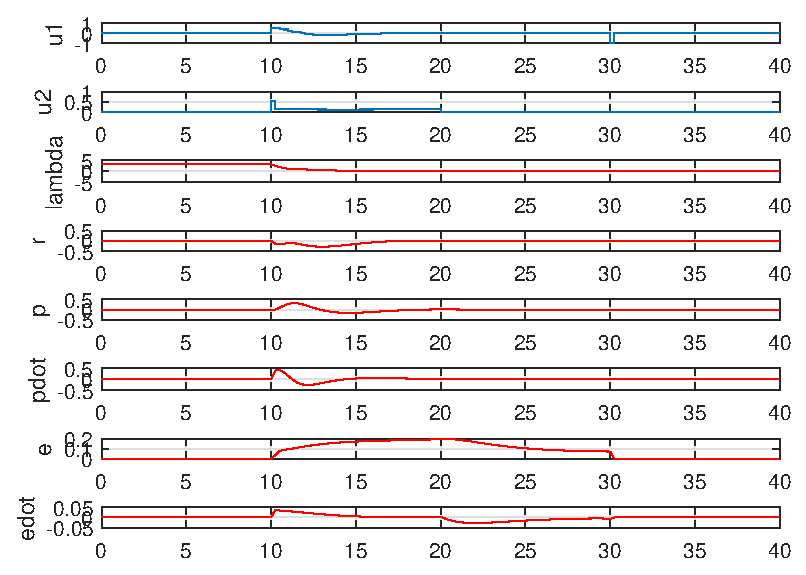
\includegraphics [width=4in]{code43_01.eps}


\subsection*{LQR}

\begin{verbatim}
Q_LQR = [1 0 0 0 0 0; 0 1 0 0 0 0; 0 0 1 0 0 0; 0 0 0 1 0 0; 0 0 0 0 1 0; 0 0 0 0 0 1 ];
R_LQR = [0.1 0; 0 0.1];
K = dlqr(A, B, Q_LQR, R_LQR);
\end{verbatim}



\end{document}
    
